\chapter{Requisiti Funzionali}
\label{ch:requisitiFunzionali}

Di seguito vengono riportati i requisiti funzionali (\texttt{RF}) del programma "SatisTrento" tramite \textit{Use Case Diagram} (\texttt{UCD}) progettati usando il linguaggio \texttt{UML}.

% Esempio di markup
\section{\underline{Utente Anonimo}}
    Di seguito i requisiti associati all'Utente Anonimo:
    \begin{itemize}
        \item \textbf{RF1}: Mappa
        \item \textbf{RF2}: Multi lingua
        \item \textbf{RF3}: Accesso dati zona selezionata
        \item \textbf{RF4}: Accesso dati specifici zona selezionata
    \end{itemize}
    \begin{figure}[H]
        \centering
        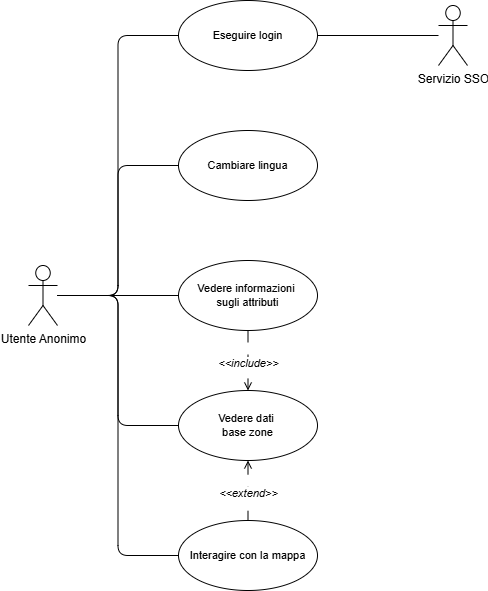
\includegraphics[width=0.8\textwidth]{UseCase_diagrams/Utente_Anonimo.drawio.png}
        \caption{Use Case Diagram dell'Utente anonimo}
    \end{figure}

    \subsection{Use Case {RF1}: Mappa}
        \subsubsection{Riassunto}
            Questo Use Case descrive come l'utente potrà interagire con la mappa
        \subsubsection{Descrizione}
            \begin{itemize}
                \item L'utente anonimo posiziona il cursone all'interno dello spazio dedicato alla mappa
                \item L'utente utilizza la rotella del mouse oppure uno dei pulsanti prensenti in uno degli angoli della mappa
                \item Il sistema ingrandisce o diminuisce la dimensione dello zoom
                \item L'utente preme e trascina il cursore
                \item Il sistema sposta il focus centrale all'interno della mappa
            \end{itemize}
        \subsubsection{Estensioni}
            Estensioni del requisito uno    % Da discutere il concetto dell'estensione per quanto riguarda l'RF2

    \subsection{Use Case {RF2}: Multi lingua}
        \subsubsection{Riassunto}
            Questo Use Case descrive come l'utente potrà cambiare la lingua dei vari testi presenti nel programma
        \subsubsection{Descrizione}
            \begin{enumerate}
                \item L'utente preme su di una delle bandiere presenti nella header
                \item La pagina si ricarica con i testi nella lingua selezionata e mette in evidenza la bandiera con la lingua corrente
            \end{enumerate}
        \subsubsection{Eccezioni}
            \begin{enumerate}
                \item Nel caso in cui l'utente anonimo selezionasse la lingua già selezionata, il sistema non deve fare nulla 
            \end{enumerate}

    \subsection{Use Case {RF3}: Accesso dati zona selezionata}
        \subsubsection{Riassunto}
            Questo Use Case descrive come l'utente potrà selezionare la zona di preferenza all'interno della mappa
        \subsubsection{Descrizione}
        \begin{itemize}
            \item L'utente anonimo preme una delle zone all'interno della visuale della mappa
            \item Il sistema 
            \item Il sistema seleziona la zona cliccata portando l'utente alla visualizzazione della zona selezionata
        \end{itemize}
        \subsubsection{Eccezioni}
            \begin{enumerate}
                \item Se l'utente clicca su di un quartiere già selezionato questo riporterà alla visualizzazione della Homepage (RF1)
            \end{enumerate}
        \subsubsection{Estensioni}
            Estensioni del requisito uno    % Da discutere il concetto dell'estensione per quanto riguarda l'RF2